%  /  significa lugares onde tem coisa para dar replace
%  ?? lugares onde estou em duvida.

%Placa
Foi desenvolvida uma nova placa para conexão ao Arduino (\textit{shield}),na qual os seguintes sensores estão dispostos: giroscópio, acelerômetro, GPS e sonar, e ainda um servo motor. A placa foi desenvolvida visando a facilidade e flexibilidade de mudanças no robô, e por isso optou-se por utilizar uma placa perfurada no lugar de um circuito impresso. 

%Sensores
Os sensores utilizados no projeto foram:
\begin{compactitem}
	\item ADXL362 Acelerômetro ~\cite{acelerometro}.
	\item L3G4200D Giroscópio ~\cite{giroscopio}.
	\item GTPA010 GPS ~\cite{gps}.
	\item Sensor Ultrassônico HC-SR04 ~\cite{sonar}.
\end{compactitem}

Com o intuito de facilitar uma futura integração dos dados do acelerômetro e do giroscópio com a navegação autônoma foram definidas APIs (\textit{Application Program Interfaces}) para cada sensor, exceto para o GPS, para o qual foi utilizada uma biblioteca já existente de nome \textit{TinyGPS} \cite{tinyGPS}. Todos os dados obtidos através dos sensores são transmitidos para o computador e publicados em tópicos definidos e, portando, disponíveis ao \textit{framework} ROS. O sonar auxilia na navegação e detalhes da sua utilização e resultados encontram-se na seção ~\ref{sec:result:slam}.

%Motor
O servo motor, modelo MG996R,  é o único atuador presente na placa, e possui a função de rotacionar o Kinect no eixo horizontal. O código implementado se baseia em uma máquina de estados tendo 3 estados possíveis: parado, rotação horária e anti-horária. Estes dados estão disponíveis para o \textit{framework} ROS, assim é possível modificar o estado do algoritmo e acessar a posição atual do Kinect a partir de outro programa que utilize o mesmo \textit{framework}. Para o SLAM e também para o OctoMap (que gera visualização 3D) a posição do Kinect pode ser alterada, mas é preciso informar ao ROS a nova posição do Kinect para que os dados obtidos deste sejam transformados para o novo sistema de coordenadas e continuem coerentes. Foi utilizado o modo \textit{sweep} para o SLAM e também para gerar o ambiente 3D, seus resultados estão nas seções ~\ref{sec:result:octomap} e ~\ref{sec:result:slam}

A API desenvolvida para os sensores consiste basicamente em fazer a leitura dos dados e a escrita deles no respectivo tópico no ROS. Assim, na inicialização dos sensores são configurados os parâmetros desejados e no \textit{loop} principal os dados são lidos e em seguida escritos em seus tópicos.

Já para o motor, a rotina inicial coloca-o na posição 0 (centro) e no estado parado. Em seguida é configurado o temporizador do Arduino para que a cada $25 ms$ o motor atualize sua posição, proporcionando assim um movimento suave. A direção do movimento é determinada pelo programa do Wiimote (sendo executado no ROS). Este programa escreve em um tópico o estado (direção) do movimento e a rotina principal no Arduino lê o mesmo tópico. O fluxograma da Figura \ref{fig:flowchartProgramaArduino} mostra como o programa do Arduino está organizado.

\begin{figure}[H]
\centering
  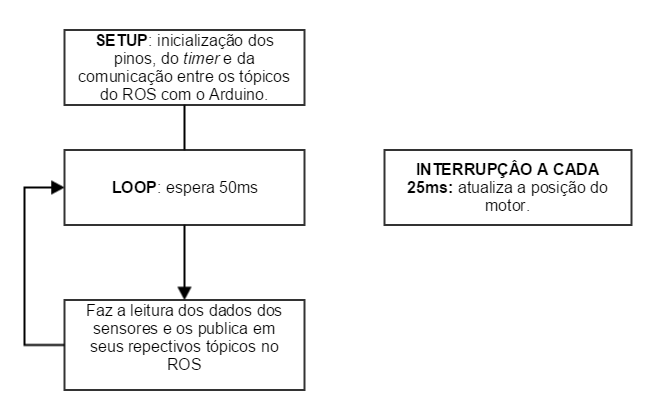
\includegraphics[scale=.5]{images/programaArduino.png} 
\caption{\small{Diagrama de fluxo para o programa executado no Arduino.}}
\label{fig:flowchartProgramaArduino}
\end{figure} 